\documentclass[a4paper,10pt]{report}

\usepackage[utf8]{inputenc}
\usepackage[english]{babel}
\usepackage[T1]{fontenc}
\usepackage{mathpazo}

\usepackage[colorlinks=true]{hyperref}
\hypersetup{urlcolor=black,linkcolor=black,citecolor=black}

\usepackage{enumerate}

\usepackage{fullpage}
\setlength{\parindent}{0pt}
\setlength{\parskip}{\medskipamount}

\usepackage{amsmath}
\usepackage{amssymb}
\usepackage{mathrsfs}
\usepackage{amsthm}
\usepackage{array}
\usepackage{graphicx}
\usepackage{comment}
\usepackage{pgfgantt}
\usepackage{soul} % highlight text

\definecolor{bluec}{rgb}{0.7, 0.7, 1.0}


\title{Projet Pensées Profondes\\\large Midterm report}
\author{
\includegraphics[width=0.3\textwidth]{../logo_ensl.pdf}\\[50pt]
Computer Science Master 1\\September 2014 \--- December 2014\\[50pt]
Mentor: Eddy \textsc{Caron}\\[50pt]
\begin{minipage}{0.4\textwidth}
    \begin{flushleft} \large
        Marc \textsc{Chevalier}
        \\
        Raphaël \textsc{Charrondière}
        \\
        Quentin \textsc{Cormier}
        \\
        Tom \textsc{Cornebize}
    \end{flushleft}
\end{minipage}
\begin{minipage}{0.4\textwidth}
    \begin{flushright} \large
        Yassine \textsc{Hamoudi}
        \\
        Valentin \textsc{Lorentz}
        \\
        Thomas \textsc{Pellissier Tanon}
        \\
    \end{flushright}
\end{minipage}
}
\date{}
\vfill

\begin{document}
\maketitle



\tableofcontents

\chapter*{Introduction}
The {\em Projet Pensées Profondes} (Deep Thought Project) aims at
providing a powerful software for answering questions written in
natural language.
To accomplish this, we developped an eponymous set of tools that
accomplish different tasks and fit together thanks to a protocol
we developped.

These various tasks include data querying (using the young and open
knownledge base Wikidata), question parsing (using the
CoreNLP software written by Stanford University and machine learning),
requests routing, web user interface, and feedback reporting.

Given the young age of this projet, these pieces are only starting
to emerge with their first features and mutual communications,
so we will describe them separately in this document without
much of a general overview of the project.


\chapter{Datamodel and communication}
We describe the choices we did about representation of the data and communication between modules.

\section{Data model}
\label{rdf}

First, we present the data model. All normalized structures of the PPP are JSON-serializable, i.e. they are trees made of instances of the following types:
\begin{itemize}
    \item \texttt{Object}
    \item \texttt{List}
    \item \texttt{String}
    \item \texttt{Number}
    \item \texttt{Boolean}
    \item \texttt{Null}
\end{itemize}

We chose to represent all normalized data as trees. To represent sentences, we have 4 kinds of nodes.

\begin{itemize}
    \item \texttt{sentence}: a question in natural language like "Who is George Washington?".
    \item \texttt{resource}: a leaf containing any kind of data (string, integer\ldots).
    \item \texttt{missing}: a leaf which marks missing values.
    \item \texttt{triple}: a 3-ary node:
        \begin{itemize}
            \item \texttt{subject}: what the triple refers to
            \item \texttt{predicate}: denotes the relationship between the subject and the
  object
            \item \texttt{object}: what property of the subject the triple refers to
        \end{itemize}         
\end{itemize}

For example, the work of the question parsing module is to transform 
\begin{verbatim}
{
    "type": "sentence", 
    "value": "Who is George Washington?"
}
\end{verbatim}
into 
\begin{verbatim}
{
    "type":
        "triple",
    "subject":{
        "type": "resource",
        "value": "George Washington"
    },
    "predicate":{
        "type": "resource",
        "value": "identity"
    },
    "object":{
        "type": "missing"
    }
}
\end{verbatim}

This structure has been chosen for its good adaptability. For instance, we can add other kind of nodes such as intersection, union, node for yes/no questions (triples without missing son), boolean operations etc..

As every tree which has ordered children, we can represent them as a string. We chose the order of the different fields in the implementation: subject, predicate, object.

To print these tree in the user interface, we do not print explicitly the \texttt{resource} nodes. A \texttt{missing} node is symbolized by a "\texttt{?}" possibly followed by an id (an integer).

For instance, the previous tree will be represented by the string:
\begin{verbatim}
(George Washington, identity, ?)
\end{verbatim}

\section{Communication}

Modules communicate with the core via HTTP requests.

The core sends them a JSON object, and they return another one.

The basic idea is that the core iterates requests to modules, which return a simplified tree, until the former gets a complete response.

During these exchanges, we keep a trace of the different steps between the original request and the current tree. The structure of a trace is a list of such trace items:
\begin{verbatim}
{
    "module":
        "<name of the module>", 
    "tree":{
        <answer tree>
    },
    "measures":{
        "relevance": <relevance of the answer>,
        "accuracy": <accuracy of the answer>
    }
}
\end{verbatim}

The measure field contains two values: relevance and accuracy.

\begin{itemize}
    \item \texttt{accuracy} is a self-rating of how much the module may have correctly understood (ie. not misinterpreted) the request/question. It is a float between 0 and 1.
    \item \texttt{relevance} is a self-rating of how much the tree has been improved (i.e. made its way from a question to an useful answer). A positive float (not necessarily greater that 1; another module might use it to provide a much better answer).
\end{itemize}

This form allows each module to access to the previous results, particularly to the user's request. The objects for request and response contains few more information such that the language used.

The data model have been implemented in a nice set of objects in both \href{http://github.com/ProjetPP/PPP-datamodel-Python}{Python} and \href{http://github.com/ProjetPP/PPP-datamodel-PHP}{PHP} in order to help the write of modules.

We could define a linear representation for the trace, using the representation of the datamodel, but it is not relevant. Indeed, this information will never be printed on the user interface.

\begin{figure}[!ht]
% https://docs.google.com/drawings/d/1toUH24GqwtpvKV7S5gje6GBxfa13R3mxgm8WlAFc_0g/edit?usp=sharing
  \centering
    \label{struct}
    \caption{Architecture of the PPP}
    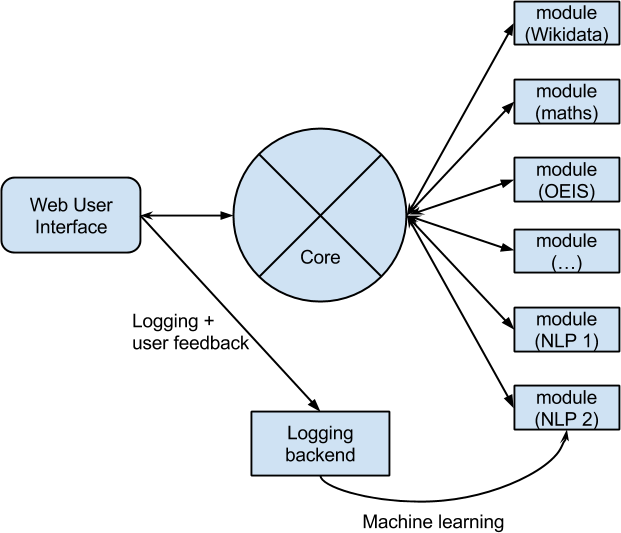
\includegraphics[width=0.5\textwidth]{../ppp_structure.png}
\end{figure}


\chapter{Core}
\section{Communications}

As its name suggests, the core is the central point of the PPP. It is
connected to all other components — user interfaces and modules — through
the protocol defined above.

The core communicates with the user interfaces and the modules {\em via} HTTP:
each time the core receives a requests from an interface, it forwards it
to modules, using a configurable list of URL where to reach modules.

An example configuration is the one we use on the production server:

\begin{verbatim}
{
    "debug": false,
    "modules": [
        {
            "name": "nlp_classical",
            "url": "http://localhost:9000/nlp_classical/",
            "coefficient": 1
        },
        {
            "name": "flower",
            "url": "http://localhost:9000/flower/",
            "coefficient": 1
        },
        {
            "name": "wikidata",
            "url": "http://wikidata.ppp.pony.ovh/",
            "coefficient": 1
        }
    ]
}
\end{verbatim}

The current state is the the Core is successfully able with all modules
that have been written: the Wikidata module, an example Python module
(which answers the question  “Who are you?”), and the Natural Language
Processing module.

\section{Routing}

Besides from communicating with other pieces of the PPP, the Core will
also route requests in such a way the power of the modules can be
combined to give something greater.

For instance, when a user will input a question like “Who is the first
president of the United States?”, the Core will send the question to
all modules and get a parsed tree from the Natural Language Processing
module. Then, it will forward this answer to all other modules, which the
Wikidata module will be able to answer.

This part is not implemented, but will be next step in the implementation
of the Core.


\chapter{User interface}
\chapter{User Interface}

We decided to implement first only a web user interface. This interface
is only composed of one web-page developed in HTML 5 with some
pieces of JavaScript and CSS. We have taken care of having an
interface that fit nice on both huge screens of desktop computers
and small screens of phones.

TODO: screenshot 

It is composed of only one huge text input with a button to submit
the query and an other one to get a random question. The text area
allows both the input of questions in English or directly of triple using
an easy notation like \texttt{(Douglas Adam, birth date,?)} to find the
birth date of Douglas Adam. A small parser written in JavaScript convert
this easy to use notation into the standard format.

In order to build this interface we have relied on some famous libraries 
ike \href{http://jquery.com/}{jQuery} and \href{http://getbootstrap.com/}{Bootstrap}.

\section{Logging}

We decided to log all requests made to the PPP to improve our algorithms,
and particularily to feed the results to Natural Language Processing
modules that use Machine Learning.
We may also use it to improve the way the Core routes/sorts answers
from the different modules, either manually or with some basic
Machine Learning.

The main idea is to log user feedback in addition to the requests
themselves: after showing the user the way we interpreted their
question alongside the answer to their request, we provide them a
way to give us feedback.
What we call feedback is actually a thumb up / thumb down pair of
buttons, and, if the latter is pressed, a way to correct the requests
parsing result so it can be fed to the Machine Learning algorithms.

Since Machine Learning algorithms are not ready yet, we did not focus
on this feature of the user interface and thus it is not implemented;
so far we only started implemented a backend that stores data
(gathered via the user interface) to a SQLite database.


\chapter{Wikidata module}
\Wikidata module is our main proof of concept module which aims to demonstrate the ability of our framework to allow the easy creation of huge modules able to answer to thousand of questions. This module tries to answer to general knowledge using the data stored in \href{http://www.wikidata.org}{\Wikidata}.

\Wikidata is a free knowledge base hosted by the \Wikimedia as a sister project of \Wikipedia. It aims to build a free, collaborative, multilingual structured database of general knowledge (for more information see \cite{42240}). It provides a very good set of API that allows to consume and query \Wikidata content easily. \Wikidata is built upon elements (called items) that are about a given subject. Each item has a label, a description and some aliases to describe it and statements that provides data about this subject.

The \Wikidata module has been written in PHP in order to rely on good libraries that allow to easily interact with the \Wikidata API. Some contributions to these libraries have been done to make them fit better with the module use case. This module works in tree steps:
\begin{enumerate}
    \item It maps \texttt{resource} nodes of the question tree into \Wikidata content: the subjects of \texttt{triple} nodes are mapped to \Wikidata items, predicates to \Wikidata properties and objects to the type of value that is the range of the \Wikidata property of the predicate. If more than one match are possible, a tree per possible match is output.
    \item It performs queries against \Wikidata content using the previously done mapping to reduce as much as possible trees. When we have a \texttt{triple} node where the object is missing the module gets the \Wikidata item of the subject, looks for values for the predicate property and replace the \texttt{triple} node with a \texttt{resource} node for each value of the triple (and so builds as many trees as there are values). When there is a \texttt{triple} node with a missing subject the module uses the \href{http://wdq.wmflabs.org}{WikidataQuery} tool API with \href{https://github.com/ProjetPP/WikidataQueryApi}{a standalone wrapper} built for the project that returns all items with a given statement.
    \item It adds clean text representation of \texttt{resource} nodes added by the previous phase.
\end{enumerate}

The global architecture of the module has been quickly studied by one of the \Wikidata developers that found it fairly good.


\chapter{Question parsing}

The goal of this module is to transform questions into trees of triples, as described in section \ref{rdf}, which can be handled by backend modules.

The difficulty of this task can be illustrated on the following example: 
\begin{center}
 \textit{What is the birth date of the president of the United States?}
\end{center}

A first possible tree is: \hl{(?,birth date, president of the United States)}. However, this tree is difficult to handle by databases-querying modules. Indeed, the ``president of the United States'' occurence in a database probably does not contain the birth date of the current president. 

On the other hand, the following tree is much more easy to process : \hl{(?,birth date, (?,president of, United States))}. In this case, the president of United States is identified (\hl{Barack Obama}), the triple becomes \hl{(?,birth date, Barack Obama)}, and finally the answer can be found easily in ``Barack Obama'' occurence.

Our goal is to product simplified and well structured trees, without losing relevant informations of the original question. We are developing three different approaches to tackle this problem. The first tries to analyze the grammatical structure of questions, the two other ones are based on machine learning.
\section{Grammatical approach}

Trees of triples can be produced after analysing the grammatical structure of sentences. First, we  present the tool we use to extract grammatical dependencies. Then, we expose chronologically our algorithm to product triples from grammatical structure.

We will detail throughout this section our algorithm on the example:
\begin{center}
 \textit{What is the birth date of the president of the United States?}
\end{center}

%########################################################################################%

\subsection{\Stanford}

The \Stanford library \footnote{\url{http://nlp.stanford.edu/software/corenlp.shtml}} is a tool developed by the \emph{Stanford Natural Language Processing group}, composed of linguists and computer scientists. This software is well-documented and considered as a ``state of the art'' tool. Moreover, it includes very efficient grammatical parsers.

Since this library is written in Java, and our module in Python, we use a Python wrapper\footnote{\url{https://bitbucket.org/ProgVal/corenlp-python/overview}} we first patched to support Python 3 and some features the wrapper did not implement.

We use \CoreNLP mostly to get grammatical dependency trees from input questions. It consists in trees which nodes are the words of the sentence, and edges reflect the grammatical relations between words.

Figure \ref{tree_one} provides an overview of such a tree on our question example \emph{What is the birth date of the president of the United States?}. For instance, the edge:
  \[\texttt{president}\xrightarrow{\texttt{det}}\texttt{the}\]
means that \emph{the} is a determiner for \emph{president}.

\begin{figure}
  \centering
  \caption{Dependency tree}
  \label{tree_one}
    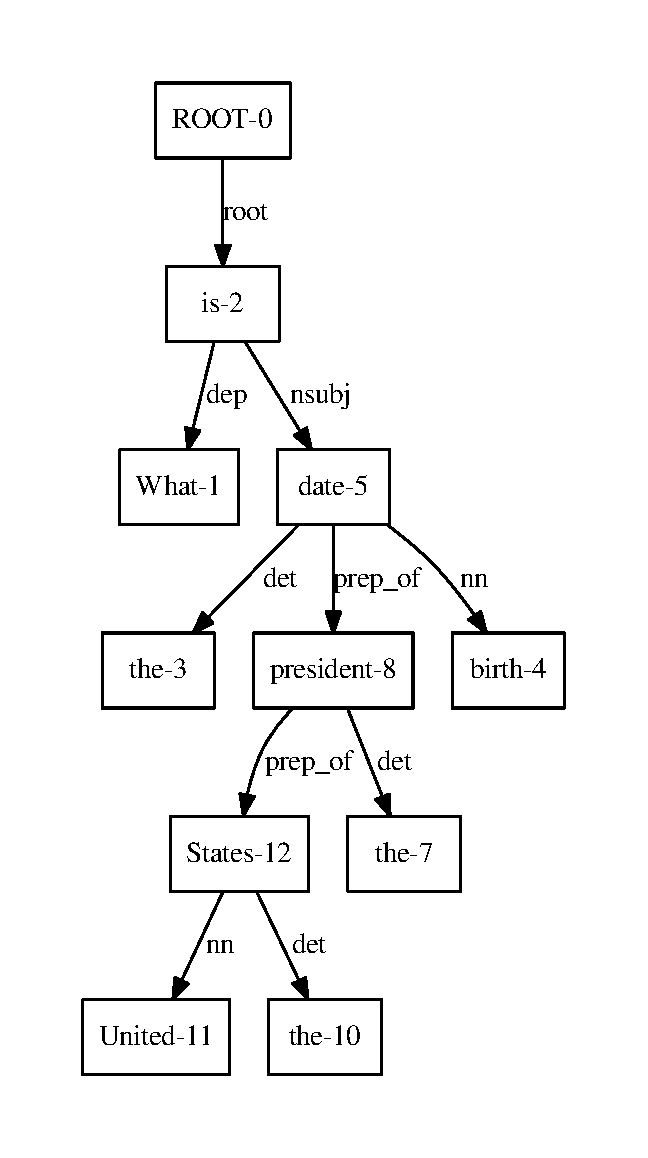
\includegraphics[scale=0.6]{../examples_NLP_grammatical/tree1.pdf}
\end{figure}

Some nodes of this tree are also endowed with tags. For example, \emph{United} and \emph{States} have the tag \emph{location}.

The Stanford typed dependencies manual (\cite{stanfordDep}) provides a full list and description of possible grammatical dependencies.

%########################################################################################%

\subsection{Preprocessing}

The preprocessing consists in a sequence of operations executed on the tree outputs by the \Stanford library. The aim is to simplify it, by merging the nodes which should belong together.

The current version of the module performs two sorts of merges:
\begin{itemize}
    \item \textbf{Merge quotation nodes.} This operation merges all the nodes which are in a same quotation (delimited by quotation marks). It also adds the words
    of the quotation which were deleted by the \Stanford library (e.g. \emph{in}, \emph{of}\dots). The final result is a node, containing the
    exact quotation, and placed at the appropriate position in the tree.
    
    \item \textbf{Merge named entities.} The \Stanford library performs a \emph{named entities recognition} (NER), which provides informative 
    tags in some nodes. For instance, \emph{United} and \emph{States} are tagged \emph{LOCATION} (see figure \ref{tree_two}). In the preprocessing step, we merge all neighbour nodes with a same NER tag. In our example, we merge the two nodes \emph{United States} into one single node.
\end{itemize}

The preprocessing also identifies the question word (Who, What, Where...) and removes it from the dependency tree.

Preprocessing is illustrated on figure \ref{tree_two}. The question word is \textit{What}.

\begin{figure}
  \centering
  \caption{Dependency tree preprocessed}
  \label{tree_two}
    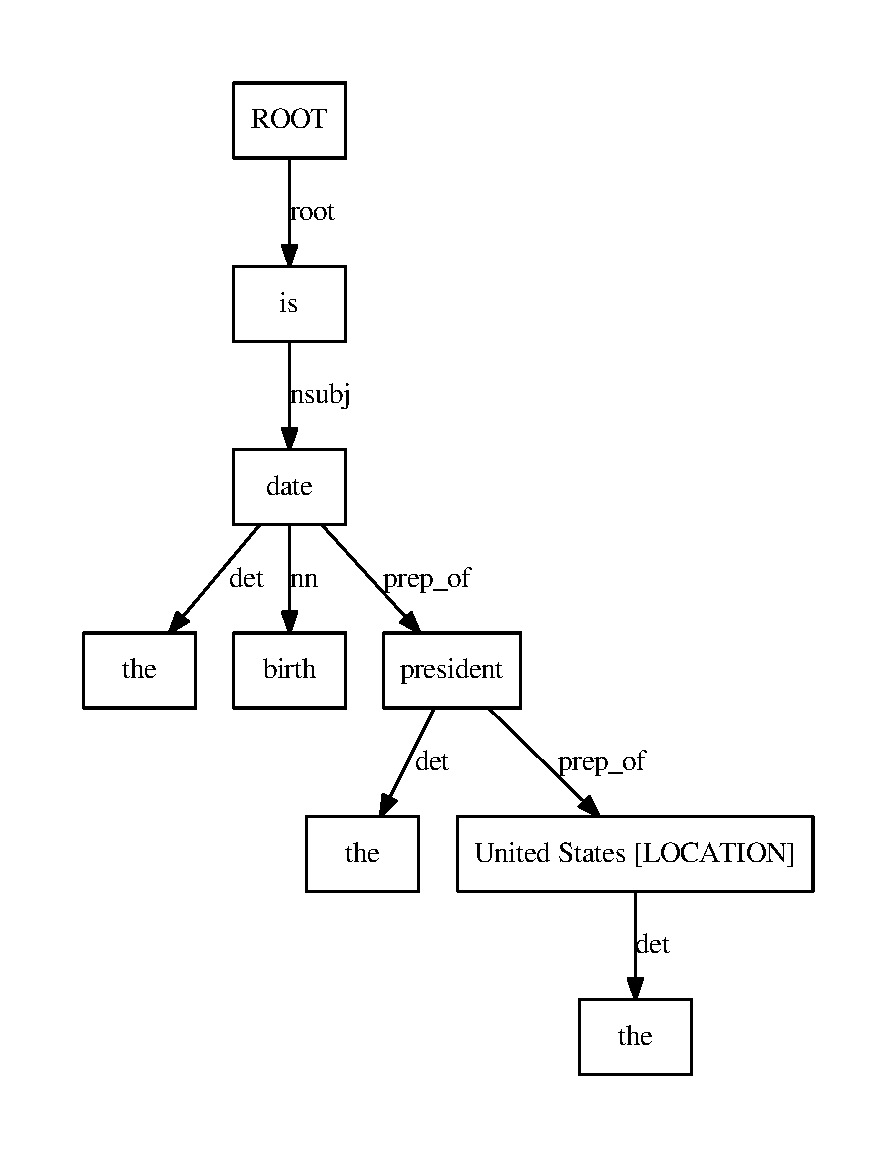
\includegraphics[scale=0.6]{../examples_NLP_grammatical/tree2.pdf}
\end{figure}

%########################################################################################%

\subsection{Grammatical dependencies analysis}

The grammatical tree is simplified by applying one of the following rules to each edge:
\begin{itemize}
 \item remove the edge and its endpoint node. For instance, a \textit{dep} relation, such as \textit{the} in our example, is often removed.
 \item merge the two nodes of the edge. Merge operations try to gather words of a same expression (e.g. phrasal verbs) that have not been merged during preprocessing.
 \item tag the edge with a ``triple production rule''.
\end{itemize}

The third operation is the most important. Dependencies relations are replaced by a restricted set of tags that will enable us to product a triples tree thereafter.

On our example, the edge:
\[\texttt{birth}\xrightarrow{\texttt{nn}}\texttt{date}\]

is merged into a single node : \textit{birth date}.

One of the triples production rules tag is : 

\[\texttt{is}\xrightarrow{\texttt{t1}}\texttt{birth date}\]

The simplified tree of our example is illustrated on figure \ref{tree_three}.

\begin{figure}
  \centering
  \caption{Dependency tree simplified}
  \label{tree_three}
    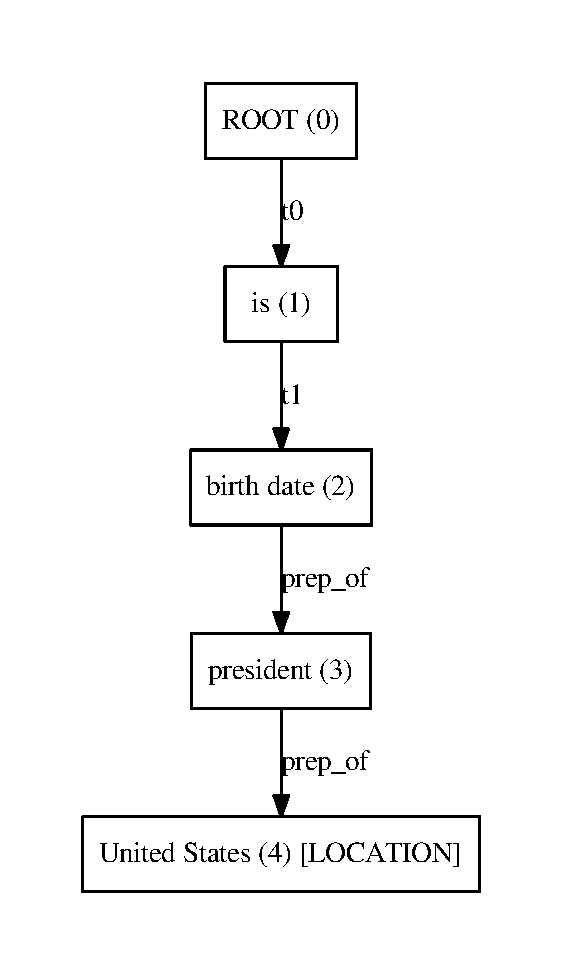
\includegraphics[scale=0.6]{../examples_NLP_grammatical/tree3.pdf}
\end{figure}

%########################################################################################%

\subsection{Triples production}

The triples production is the final step. It outputs the triples tree.

First, we assign a number to each remaining node. The root of the tree has always number \textit{0}. We have directly print these numbers on figure \ref{tree_three}.

Then, we associate to each subtree of root's number \textit{x} an unknown denoted \textit{?x} that identifies the information the subtree refers to. On our example, the subtree of root \textit{president} (number \textit{3}) represents the name of the president of the United States. This unknown is denoted \textit{?3}.

Unknowns are linked together into triples thanks to the triples production rules tagged previously. For instance, an  edge tagged \textbf{t2}:

\[\texttt{a}\xrightarrow{\texttt{t2}}\texttt{b}\]

products the triples \hl{(?a,a,?b)}, or \hl{(?a,a,b)} if b is a leaf (a and b are replaced by the words of the node they refer to).

The tag \textbf{t1} directly linked two unknowns \hl{?a = ?b}, instead of producing a triple.

The tag \textbf{t0} products nothing.

We obtain the following result on our example:

\begin{center}
 ?1 = ?2 ~\\
 (?2 , birth date of , ?3) ~\\
 (?3 , president of , United States)
\end{center}

Then, we link \textit{?0} to \textit{?1}, depending on the question word of the question. Here we have (question word \textit{What}):
\begin{center}
 (?1,definition,?0)
\end{center}

The four previous rules are simplified in a set a triples:

\begin{center}
 (?1,definition,?0) ~\\
 (?1 , birth date of , ?3) ~\\
 (?3 , president of , United States)
\end{center}

Find an answer to the question is equivalent to build a model of the conjunctive formula: \textbf{(?1 , definition , ?0)$\wedge$(?1 , birth date of , ?3)$\wedge$(?3 , president of , United States)} and outputs the value of \textit{?0}.

The triples tree is obtained by replacing each unknown \textit{?x} by a triple containing \textit{?x} \textit{and not} \textit{?0}. The final result, taken from the PPP website, is printed on figure \ref{tree_four}. Figure \ref{triple_tree} contains the formal representation of the triples tree of our example.

\begin{figure}[!h]
  \centering
  \caption{Triples tree}
  \label{tree_four}
    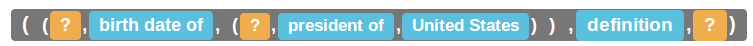
\includegraphics[scale=0.5]{../examples_NLP_grammatical/final_result.png}
\end{figure}

Backend modules (such as Wikidata module) will have to fill intermediate unknowns : \hl{((August 4 1961,birth date of, (Barack Obama, president of, United States)), definition, ?)} and finally provide the final answer that replaced \textit{?} (for example: a description of the August 4 1961 date).


%########################################################################################%

\subsection{Future work}

\subsubsection{Grammatical rules analysis}

Our analysis of grammatical rules, in order to product triples, is very basic. Currently, we only have about 5 rules. Although it is good enough to handle a lot of questions, we are not able to process conjunctions for example (e.g. \textit{``Who wrote "Lucy in the Sky with Diamonds" and "Let It Be"?''}).

\subsubsection{Preprocessing merging}

There remains nodes which should stay together but are not merged by our module, for instance \emph{prime minister} or \emph{state of the art}. Recognizing such words is called \emph{Multiword Expressions Processing}. This task is a whole part of Natural Language Processing theory. 

We have several tracks to improve merging. Existing algorithms or softwares need to be tested. We could also use multiword expressions dictionaries.

\subsubsection{Question type analysis}

The current algorithm attaches great importance to the type of the input question. Sentences starting by a question word (Who, Where, How ...) are better processed than Yes/No questions for instance.

\subsubsection{Triples tree improvement}

The triples tree will be improved to take into account new types of nodes, adapted to databases queries. For example, a node could be tagged ``FIRST'' to pick the first occurrence of a list of answers (e.g. \hl{FIRST(?,presidents of, United States)}).

\section{Reformulation : a learning approach }

Efficiency of neural network nowadays can be very good. An approach based on network is also used here. But, the aim is not to learn answering question, there are two reasons for that: first the knowledge changes over time, e.g. the president name depends of the date, then something simple is wished, the learning process should also be continuous. In the second case, learning the answer implies to know proper Names which increase the size of the dictionary, that means the learning time. The module presented here try to reformulate a question. In fact it try to translate the question for the wikidata module.

\subsection{How it works}

There is a output of the grammatical module which builds a triple representation of the question. All work is done on this representation. The assumption ``all useful information is keep in this form''  is also necessary. The module has also a dictionary. There are four step to do. First a pretreatment replace proper names and numbers with tags, such that all word of the triple are in the dictionary, then the request is projected in the math space of request. Two last step reveres the two first, but the reverse projection should produce a better request, which mean the final request is adapted for the Wikidata module.

\subsubsection{Mathematical spaces}

The mathematical space of request $\mathcal{R}$ is simply the subset of the $\mathbb{R}$ vector space of dimension 50, were all vector have an euclidean norm of 1.
A triple is formed of a subject request, a predicate and an object request, it is also natural to consider the triple over $\mathcal{R}$, and matching will always follow the order subject, predicate, object.
Let us call vector the elements of $\mathcal{R}$.
The choice of a 50-dimension can be modified if necessary, but taking a higher dimension could slow the learning process, and with a lower space we could lost some expression power, which may lead to very poor results.

%To unify everything As we works with requests, we consider everything is a request, even a word.

%There are 2 generic spaces: the one of words which is a vector space of dimension 50 and the space of request which is the space of word triples. The first word of a triple represents the subject, the second represents the predicate and the last the object.
%To distinguish words which are vectors and words with letters, we will add the adjective English to the seconds.

\subsubsection{Dictionary}

The dictionary defines matching between English words and vectors triple, which is the base of the process. We use triple because a word could have different meaning depending on his nature, so predicate vector for a word is not the same as subject vector which is not the same as object vector. We will denote m.s vector-subject of word m, m.p and m.o for predicate and object.

\subsubsection{Pre- and post-treatment and treatment}

We evoke some reasons not to handle proper name directly (the dictionary size would increase and names could changes), there is another arguments: there is an arbitrary number of proper names, because you can invent some new names every time. That is why they are replace in a request by a tag NAMEi, $i\in{1,2,3}$. It allows us to have three different names in a question, and that is sufficient. The same happens for numbers. Tag UNKNOWN finally represents the ``holes'' in the request tree. At the end, after the treatment we replace tags with corresponding real names or numbers in the final tree.

Recognizing a number is not hard, in fact it is just checking it the characters sequence looks like numbers optionally followed by a dot and numbers. If the sequence is not a number or a ``hole'' and is not in the dictionary, the module treat it as a proper name.

\subsubsection{Project form a request to a vector}

The model allow an arbitrary request form, it mean we have a three with an unknown depth, and to keep the complete question information we should handle it so. But the request are triple, so it is easy to transform. First with the dictionary all word are replaced with vectors, of course we take the vector corresponding to the function of the word in the tree. Then we have to ascend the whole three to compute the root value.

Let define a matrix compact which take a triple of vector and merge them in one vector, here merging in not a intuitive operation, in fact we don't known how to merge this triple, that is why all coefficients of the matrix are unknown. To compute what we call a vector, output should be normalized.

Now by applying this operation bottom-up in the tree. Main idea is each node value represent the subtree request.


\subsubsection{Reconstruct a request from a vector}

This operation is quite symmetrical of the projection, with a matrix uncompact we can the same way obtain a vector triple from a vector, and recursively an tree appears. But the question is how to known if we should reapply the function uncompact or leave the vector as a leaf? First say in a triple predicate is never a tree, then object and subject will be let as leaf if a known word is near enough. Finally each node is replace with the nearest corresponding word of the dictionary, that mean for example for a vector in middle of a triple which is also a predicate take word with nearest predicates' vector.

Defining near enough is difficult. To avoid infinite loop we will take depth of nodes into account. We must take $\delta>0$ a precision factor and $g$ a growth factor. If $d$ is depth of node $n$, near enough means distance is bounded by $\delta*g^d$ with regard of euclidean norm.  

The algorithm is also :



\begin{algorithm}[H]
    \DontPrintSemicolon  % Some LaTeX compilers require you to use \dontprintsemicolon instead
    \KwIn{$\delta>0$ et $a\in A$}
    \KwOut{request tree}
    $(s,p,o) \gets \text{uncompact}(a)$\;
    Find m s.t. $\N{m.s-s}<\delta$ is minimal \;
    \lIf{m exists}{
        $s \gets m.s$
    }
    \lElse{
        $s \gets C(\delta,s)$
    } 
    Find m s.t. $\N{m.o-o}<\delta$ is minimal \;
    \lIf{m exists}{
        $o \gets m.o$
    }
    \lElse{
        $o \gets C(\delta,o)$
    } 
    $p \gets \underset{m}{\text{argmin}}.r (\N{m.r-m.p})$\;
    \Return{$(s,r,o)$}\;
    \caption{From vector to tree}
\end{algorithm}



\subsubsection{Remarks}

Matrix compact and uncompact are not bijective after restraining the request space to existent requests. Applying uncompact then compact should give the identity, with of course an error margin, but when compacting then uncompacting we only have to find an equivalent request, i.e. with the same meaning but with another formulation. If it were not the case it would produce exactly the same out as the input, that would be useless.

\section{Learning}

Training the model can not be done easily with a classical back-propagation because we have no idea what is the best triple for a question. The solution is also to try to change a little the matrix, and see what changes improve the best the quality of result, it is however very bad in cost. 

Now to compute the quality of result, i.e. the score  of the module we use a semantic distance: it's a norm depending of the mean of words. To be simple we base it of the relation graph ``instance of'' of Wikidata assuming it is a directed acyclic graph. We compute the nearest common ancestor and we add the distance between this node and the two word  nodes.

\subsection{Implementation}

The module is written in C++, with threads to speed up the matrix multiplication. To interface it with the others, it is build as a shared library with python library. The dictionary has been generated using the clex \footnote{\url{https://github.com/Attempto/Clex}}. 

\subsection{Future work}

Learning process is not made yet. As latency with Wikidata is very high (several seconds) we have to download Wikidata and run it in local.

Then we could think of different manners to train the model.

%Finding a way to learn everything with first or second approach is the most important, as the first answering module in functional, learning is possible. Then, learning and computation speed-up will be important, the search for nearest neighbor is long, maybe it is linear, but with near 100 000 words and high dimension it becomes consequent, use of heuristics could be a good idea, for example there exists distance sensitive hash. Kd-trees allow a search in log-time (with precomputation) ; but with dimension 50, the constant factor $2^{50}$ is too large. 


\section{Machine Learning 2}


We used machine learning algorithms in order to produce triples from scratch, i.e. without any grammatical library like \Stanford.

Motivations come from two points:
\begin{itemize}
\item Triples are linked to the semantic of the sentence, and not directly from the grammar
\item It has been shown that a machine learning approach can produce, for a large panel of different NLP problems, very good solutions, closed to \textit{state of the art} algorithms \cite{collobert}.
\end{itemize}

This work is based mainly on the paper "Natural Language Processing (almost) from Scratch" \cite{collobert}.
For the baseline, we limited ourselves to one level of depth.
For example, the sentence "What is the birth date of the president of the United States?" will be converted to the triple: 
\hl{(president of the United States, birth date, ?)}. 

We used a look up table and a window approach neural network. The complete package was written in Python 3 and in Lua, with the Torch7 library\footnote{\url{http://torch.ch/}}.

\subsection{Data set}

Because we used supervised algorithms, we need a data set of annotated questions.
This data set has to be built manually, because we did not find on internet a data set that directly answers to the problem of triple extraction.
Build this data set is a fastidious work. Currently our data set is composed of 168 questions.
Because the mean of number of words in one question in the data set is around 7.5, it gives us 1264 entries to train/test the neural network.

\subsection{Structure of the network}

For each word $w$ of the sentence, we want to classify $w$ into four categories: \textit{subject}, \textit{predicate}, \textit{object} and \textit{to ignore}.
The classification of each word of the sentence into these four categories produce the desired triple.

As described in \cite{collobert}, we used a window approach, and a look up table.

\begin{figure}[!ht]
  \centering
  \caption{The neural network architecture, as described in \cite{collobert}}
  \label{sandalone:tree_four}
    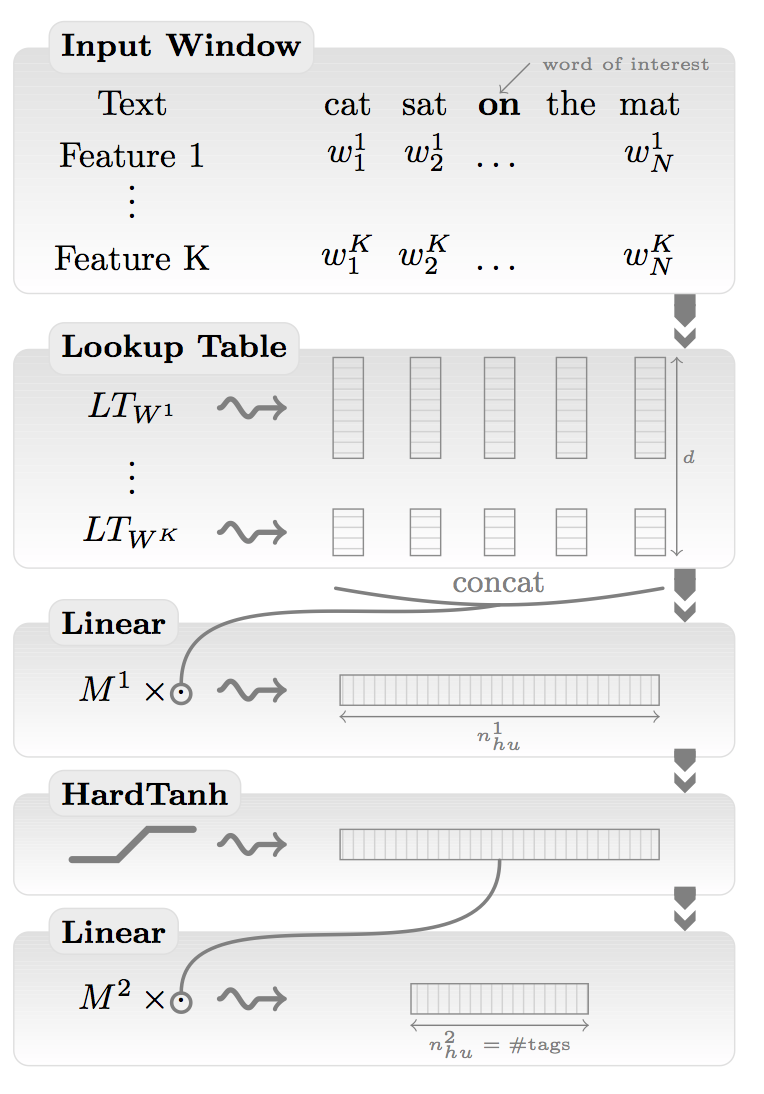
\includegraphics[scale=0.5]{../NLP-standalone-images/network.png}
\end{figure}

\subsubsection{Window approach}

We used a window that focuses on the word to classify. For example, if the sentence is "What is the birth date of the president of France?", and the word to classify is "date", for a window size of 7, the window is: "is the birth \textbf{date} of the president".

We used this window because neural networks works with a fixed number of input parameters. 
The window size is a meta parameter to choose. This window has to be large enough that we can decide in the context of the window in which category a word is. We used a window of size 7.

\subsubsection{Look up table}

The look up table is a dictionary that associates to each word $w$ a vector $V_w \in \mathbb{R}^n$, where n is the number of parameters we used to encode a word. We used $n=25$.
If two English words $w_1$ and $w_2$ are synonymous, then $||w_1-w_2||_2$ is small.

The construction of look-up table is described in \cite{collobert} and used unsupervised machine learning techniques.
We used a precomputed look up table, found here: \url{http://metaoptimize.com/projects/wordreprs/}

We also add one parameter that give us if the word starts with a capitalize character or not. Finally words are embedded in vectors of dimension 26. 

\subsubsection{The neural network}

We tried two different architectures:
-A linear model, i.e. without any hidden layers. This gives us $26\times 7\times 4 = 728$ parameters to optimize. 
-A non linear model with one hidden layer of size 10. This gives us $26\times 7\times 10\times 4 = 7280$ parameters to optimize.

The linear model has the advantage to have few parameters, so it can be learned with a small data set of annotated questions. However we found that this model is not enough powerful to catch the complexity of the problem we want to solve.
The non linear model is more complex and can describe with more precision how the English language works. But because of the huge number of parameters to learn, we need a larger annotated data set that we currently have.

We add one regularization parameter to limit over-training.
The neural network is implemented in Lua with the Torch7 framework.
Few minutes of computation are needed to train successfully the model.

\subsection{Results}

This baseline algorithm, witch was the goal for the midterm, give us quite good results.
The linear model has an accuracy of 80\% on the training set, and the non linear model has an accuracy of 98\% on the training set.
On the test set, these two models have an accuracy of 60\%, witch is much better than chance (a random method would give us 25\% of accuracy), but it is not efficient enough to be used for tricky questions (e.g. that are not closed to one of the sentence in our annotated data set).

\subsection{Future work}

\subsubsection{Unsupervised deep learning}

We could use auto-encoders  with Restrictive Boltzmann Machine (R.B.M) and an unsupervised data set of questions to learn a much more efficient representation of a question, as explained in \cite{fischer2012introduction} and in \cite{hinton2006reducing}

We can easily found large data set of non annotated questions.
One advantage of doing this is to limit supervision (because our annotated data set is very small), and it should improve the capacity of our model to generalize to questions that are not in our data set.

\subsubsection{Used a more efficient preprocessing}

We could reuse a part of the work done in the grammatical approach to have a better input for the neural network. For example, we could use the "Merge quotation nodes" and the "Merge named entities" steps to simplify input questions.

\subsubsection{Merge the work done with the grammatical approach}

This ML approach gives us, for each word of the sentence, the probability to be in the \textit{subject}, in the \textit{predicate}, in the \textit{object} or a word to ignore.
Maybe we can use this information to improve the accuracy of the grammatical approach.




\chapter*{Conclusion}
\begin{frame}[fragile]
    \frametitle{Nested question}

Who is the wife of the president of the United States?
    \begin{tabular}{ll}
        \alert{WolframAlpha} & Barack Obama\\
        \alert{Platypus} & Michelle Obama\\
    \end{tabular}

    \medbreak

    What are the birth dates of the daughters of the wife of the president of the United States?
    \begin{tabular}{ll}
        \alert{WolframAlpha} & Barack Obama\\
        \alert{Platypus} & Saturday, July 4, 1998 \& Sunday, June 10, 2001\\
    \end{tabular}
\end{frame}

\begin{frame}[fragile]
    \frametitle{Conjunction}

Who is an actor in Titanic and Inception?
    \begin{tabular}{ll}
        \alert{WolframAlpha} & all the actors of the two movies\\
        \alert{Platypus} & Leonardo DiCaprio\\
    \end{tabular}
\end{frame}

\section{Future work}

\begin{frame}[fragile]
    \frametitle{Better database}

    ``How fast is the TGV?''

    ``How wide is a tennis court?''

    Not answered by \alert{Wikidata}.

    \medbreak

    $\rightarrow$ Improve Wikidata?

    $\rightarrow$ Use another database?
\end{frame}

\begin{frame}[fragile]
    \frametitle{Better question parsing}

    ``What is the date of birth of Isaac Newton?''

    ``In which band does Bono sing?''

    Not parsed correctly.

    \medbreak

    $\rightarrow$ Train the Stanford CoreNLP library?

    $\rightarrow$ Improve the algorithm of the Grammatical module?

    $\rightarrow$ Better datasets for the ML modules?
\end{frame}

\begin{frame}[fragile]
    \frametitle{New modules}
    \begin{table}
    \Large
    \centering
    \begin{tabular}{ccc}
        \textcolor{mLightBrown}{cooking recipes} & \textcolor{mDarkBrown}{HAL} & \textcolor{mMediumBrown}{meteo} \\
        \multicolumn{3}{c}{\textcolor{mDarkTeal}{programming language interpreter}} \\
        \textcolor{mMediumBrown}{cinema} & \textcolor{mDarkTeal}{music} & \textcolor{mLightBrown}{literature}\\
        \textcolor{mDarkBrown}{OEIS} & \textcolor{mLightBrown}{translation} & \textcolor{mDarkTeal}{chemistry}\\
        \multicolumn{3}{c}{\textcolor{mMediumBrown}{sport statistics and predictions}} \\
    \end{tabular}
    \end{table}
\end{frame}

\begin{frame}[fragile]
    \frametitle{Some facts} % to update just before the presentation
    \alert{23 repositories}

    \begin{tabular}{lll}
        6 & PHP & Wikidata libraries and module\\
        12 & Python & Other modules, core, and libraries\\
        1 & C++ & ML-Reformulation\\
        1 & Shell & Deployment scripts\\
        1 & \LaTeX & This presentation and the report\\
        1 & Markdown & The specification\\
        1 & HTML/CSS/Javascript & The Web User Interface\\
        1 & HTML/CSS & The project's website\\
    \end{tabular}

    \alert{1982 commits} (without the ``integration'' repository, which has an automatic commit every 12h)

    \alert{26k lines} of code (13k in PHP, 10k in Python)
\end{frame}

\newlength{\logosize}
\setlength{\logosize}{12pt}
\begin{frame}[fragile]
    \frametitle{Stay tuned}
    \alert{\url{http://projetpp.github.io/}}

    \begin{tabular}{ll}
        
\includegraphics[width=\logosize]{Twitter_logo_blue.png} & \href{https://twitter.com/ProjetPP}{https://twitter.com/ProjetPP}\\
        
\includegraphics[width=\logosize]{GitHub-Mark-32px.png} &  \href{https://github.com/ProjetPP}{https://github.com/ProjetPP}\\
        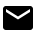
\includegraphics[width=\logosize]{ic_email_black_18dp.png} & \href{mailto:ppp@pony.ovh}{ppp@pony.ovh}\\
    \end{tabular}
\end{frame}


\begin{frame}
    \frametitle{Questions?}
    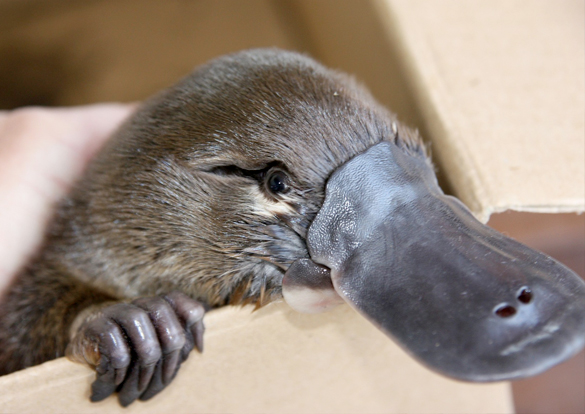
\includegraphics[width=\linewidth]{figures/platypusLg.jpg}
\end{frame}


\appendix

\bibliographystyle{alpha}
\bibliography{bibliography}
\nocite{*}

\chapter{NLP \--- Grammatical approach}

\begin{figure}
\caption{Triples in tree form}
\label{triple_tree}
\begin{verbatim}
{
    "subject": {
        "subject": {
            "type": "missing"
        },
        "type": "triple",
        "object": {
            "subject": {
                "type": "missing"
            },
            "type": "triple",
            "object": {
                "type": "resource",
                "value": "United States"
            },
            "predicate": {
                "type": "resource",
                "value": "president of"
            }
        },
        "predicate": {
            "type": "resource",
            "value": "birth date of"
        }
    },
    "type": "triple",
    "object": {
        "type": "missing"
    },
    "predicate": {
        "type": "resource",
        "value": "definition"
    }
}
\end{verbatim}

\end{figure}

\end{document}
